\chapter{Question 2}
\label{avoiding-uri-aliases} 

\textbf{Write a Python program that:
Download the TimeMaps for each of the target URIs.  We'll use the ODU Memento Aggregator, so for example:}\\
\textbf{URI-R = {\url{http://www.cs.odu.edu/}}\\
URI-T = {\url{http://mementoproxy.cs.odu.edu/aggr/timemap/link/1/http://www.cs.odu.edu/}}\\
Create a histogram* of URIs vs. number of Mementos (as computed from the TimeMaps).  For example, 100 URIs with 0 Mementos, 300 URIs with 1 Memento, 400 URIs with 2 Mementos, etc.}\\
\textbf{$*$ = https://en.wikipedia.org/wiki/Histogram}

\begin{itemize}
\item With the help of ODU Memento Aggregator, I downloaded TimeMaps for all the URIs that are extracted in question 1 using the following curl command:\\
{\url {curl -i --silent http://mementoproxy.cs.odu.edu/aggr/timemap/link/1/<uri>}}
\item  I stored the output produced by the cURL command into a file `PagesList'. 
\item I processed the data from the above file to create a JSON with the original URI, memento URI , datetime and memento count. The memento count for each URI is derived by counting the URIs with rel=``memento''. This is outlined in Listing \ref{lst:code1}.
\item Using `uri.py' I wrote the memento count for all the 1000 URIs and URIs with $>$ 0 mementos in 2 different files `allMementos' and `mementosExcluding0' respectively.This code is listed in Listing \ref{lst:code2}.
\item File `mementosExcluding0' is used for question 3 and file `allMementos' is used for plotting a histogram with memento count on x-axis and frequency on y-axis.
\item I observed that most of the URIs are not archived as they are recently created tweets. Out of 1000 instances 849 tweets have 0 mementos.
\item This distribution is summarized in Figure \ref{fig:fig1}.
\end{itemize}

\begin{figure}[h!]
\begin{center}
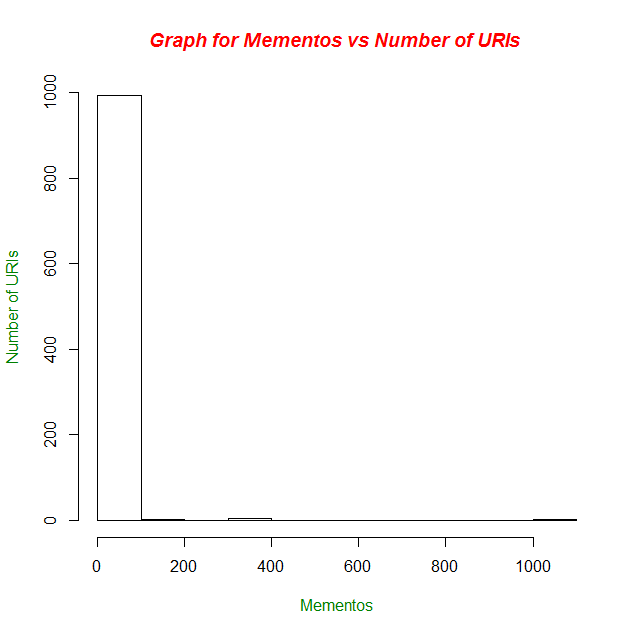
\includegraphics[scale=0.55, keepaspectratio=true]{figures/q2Graph.png}
\caption{Graph for Mementos vs Number of URIs}
\label{fig:fig1}
\end{center}
\end{figure}

\newpage
\textbf{Code Listing}
\lstinputlisting[language=Python,caption=``Python code for getting mementos data and writing the output into a json file'',frame=single,label=lst:code1,breaklines=true,captionpos=b,numbers=left,showspaces=false,showstringspaces=false,basicstyle=\footnotesize]{src/countMementos.py}

\textbf{Code Listing}
\lstinputlisting[language=Python,caption=``Python code for writing all mementos count and URIs with count $>$ 0 in 2 different files '',frame=single,label=lst:code2,breaklines=true,captionpos=b,numbers=left,showspaces=false,showstringspaces=false,basicstyle=\footnotesize]{src/uri.py}


